\usetikzlibrary{%
	chains,
	calc,
	shapes,
	decorations,
	scopes,
	arrows,
}

\tikzstyle{lane-right}=[start chain=going right,node distance=1ex]
\tikzstyle{lane-left}=[start chain=going left,node distance=1ex]

\newcommand\carangle[1]{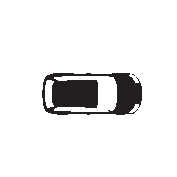
\includegraphics[height=2ex,angle=#1]{car}}
\newcommand\carr{\carangle{0}}
\newcommand\carl{\carangle{180}}

\newcommand\rsu{\includegraphics[height=6ex]{rsu}}
\newcommand\server{\includegraphics[height=6ex]{server}}

\newcommand\basicroad{%
% coordinates
\foreach \pos/\coord in {top/3ex, center/0, bottom/-3ex}{
\coordinate (\pos-left) at (0,\coord);
\coordinate (\pos-right) at (\textwidth-\pgflinewidth,\coord);
}

\coordinate (lane1-left) at (1,-1.5ex);
\path (\textwidth-\pgflinewidth,-1.5ex) +(-1,0) coordinate (lane1-right);
\coordinate (lane2-left) at (1,1.5ex);
\path (\textwidth-\pgflinewidth,1.5ex) +(-1,0) coordinate (lane2-right);

\coordinate (lane1) at (lane1-left);
\coordinate (lane2) at (lane2-right);

% basic road shape
\fill[road-fill] (top-left) rectangle (bottom-right);
\draw[road-draw] (top-left) -- (top-right);
\draw[road-draw,loosely dashed] (center-left) -- (center-right);
}

\newcommand\road{%
\basicroad
\draw[road-draw] (bottom-left) -- (bottom-right);
}

\newcommand\onramproad{%
\basicroad

% on-ramp bottom
\fill[road-fill] (bottom-left) -- ++(3,0) to[out=0,in=180] ++(1,-3ex) -- ++(3,0) coordinate (bend) to[out=0,in=135] ++(1,-3ex) -- ++(45:3ex) to[out=135,in=0] (bend |- bottom-left) -- cycle;

\draw[road-draw] (bottom-left) -- ++(3,0) coordinate (ramp-start) to[out=0,in=180] ++(1,-3ex) -- ++(3,0) coordinate (bend) to[out=0,in=135] ++(1,-3ex) ++(45:3ex) to[out=135,in=0] (bend |- bottom-left) coordinate (ramp-end) -- (bottom-right);

\draw[road-draw,dashed] (ramp-start) -- (ramp-end);
}

\newcommand\commwave[2]{%
\path[wave-fill] #1 circle (#2);
\path[wave-draw] #1 circle (#2);
}

\newcommand\accidentright{%
\accident{right}{0}
}

\newcommand\accident[2]{%
% accident

\path (lane1-#1) +(#2,0) coordinate (p1);
\path (lane2-#1) +(#2,0) coordinate (p2);

\path (p1) edge node[right,accident-star,star,minimum size=4ex] {} (p2);
\node[rotate=30] at (p1) {\carr};
\node[rotate=-50] at (p2) {\carr};
}

\newcommand\trafficjam[2]{% begin point (right), #cars
\begin{scope}[lane-left,node distance=.2ex]
	\path #1 node[on chain] {\carr};
	\foreach \i in {2,...,#2}{
	\node[on chain] {\carr};
	}
\end{scope}
}
